\documentclass[conference]{IEEEtran}
\IEEEoverridecommandlockouts

\usepackage{cite}
\usepackage{amsmath,amssymb,amsfonts}
\usepackage{algorithmic}
\usepackage{graphicx}
\usepackage{textcomp}
\usepackage{xcolor}
\usepackage{booktabs}
\usepackage{listings}
\usepackage{url}
\usepackage{hyperref}
\hypersetup{
    colorlinks=true,
    linkcolor=black,
    urlcolor=blue,
    citecolor=blue,
}

% Source code listing style
\definecolor{codegreen}{rgb}{0.0,0.5,0.0}
\definecolor{codepurple}{rgb}{0.58,0,0.82}
\definecolor{codegray}{rgb}{0.4,0.4,0.4}
\definecolor{codebg}{rgb}{0.97,0.97,0.97}
\lstdefinestyle{pystyle}{
    backgroundcolor=\color{codebg},
    commentstyle=\color{codegreen}\itshape,
    keywordstyle=\color{blue}\bfseries,
    stringstyle=\color{codepurple},
    numberstyle=\tiny\color{codegray},
    basicstyle=\ttfamily\scriptsize,
    breakatwhitespace=false,
    breaklines=true,
    captionpos=b,
    keepspaces=true,
    numbers=left,
    numbersep=4pt,
    showspaces=false,
    showstringspaces=false,
    showtabs=false,
    tabsize=2,
    frame=single,
    rulecolor=\color{codegray!40},
}
\lstset{style=pystyle, language=Python}

\def\BibTeX{{\rm B\kern-.05em{\sc i\kern-.025em b}\kern-.08em
    T\kern-.1667em\lower.7ex\hbox{E}\kern-.125emX}}
\begin{document}

\title{Lending Club Loan Default Prediction:\\
A Four-Phase Pipeline from Pandas to Conversational AI}

\author{
\IEEEauthorblockN{Aayush Nepal,~Junwei Zhang,~Lusi Zhang}
\IEEEauthorblockA{\textit{404 Team Not Found} \\
\textit{EAS 587 Spring 2026}\\
University at Buffalo \\
Buffalo, NY, USA}
}

\maketitle

\begin{abstract}
We build an end-to-end loan default prediction system on the Lending Club
2014--2017 cohort and progressively rescale the same use case across four
implementations: a local pandas pipeline, a tuned scikit-learn model, a
Spark + Delta Lake medallion architecture extended with Federal Reserve
macroeconomic data, and finally a Streamlit application paired with a
Model Context Protocol (MCP) server that exposes the trained model to
conversational LLMs. The production XGBoost model attains 0.726 AUC-ROC,
0.410 AUC-PR, and a Kolmogorov--Smirnov statistic of 0.328 on a strictly
held-out 314{,}212-loan 2017 test set. Three design choices carry the
result: a strict 21-column post-loan leakage filter, a chronological
train/validation/test split that prevents macro leakage, and an eight-stage
custom transformer pipeline that is fit on training data only and reused
verbatim by the deployment surfaces. We additionally evaluate whether
augmenting the model with seven Federal Reserve series improves predictive
lift; the experiment yields a 0.0005 AUC delta on validation, leading us to
report the macro layer's value through three stakeholder-facing insights
rather than through model performance.
\end{abstract}

\begin{IEEEkeywords}
loan default prediction, gradient boosting, leakage discipline, Spark,
Delta Lake, Model Context Protocol, scikit-learn pipelines
\end{IEEEkeywords}

% =============================================================================
\section{Introduction and Background}
% =============================================================================

Lending Club operates an unsecured personal-loan marketplace that issued more
than two million loans between 2007 and 2020. For each application the
platform computes a sub-grade between A1 (lowest risk) and G5 (highest) and
prices the loan accordingly. From a lender's perspective, the central
underwriting question is whether a given applicant will repay the principal
in full or charge off, with the loss-given-default at par because the loans
are unsecured. Phase 4 of this project is the culmination of a semester-long
effort to answer that question end-to-end.

The contribution of this paper is not a single model but the deliberate
\emph{evolution} of a single use case across four implementations. Phase 1
performs the data foundation work in pandas. Phase 2 produces a tuned
scikit-learn pipeline whose XGBoost classifier is the production artifact.
Phase 3 rebuilds the data layer on Spark + Delta Lake using the medallion
pattern and adds a Federal Reserve macro overlay. Phase 4 deploys the same
trained pipeline two ways: through an interactive Streamlit application and
as a Model Context Protocol (MCP) tool inside Claude Desktop. Each
implementation reuses the artifacts of the previous one rather than
restarting the modelling work. Figure~\ref{fig:architecture} summarises the
overall pipeline.

\begin{figure}[t]
\centering
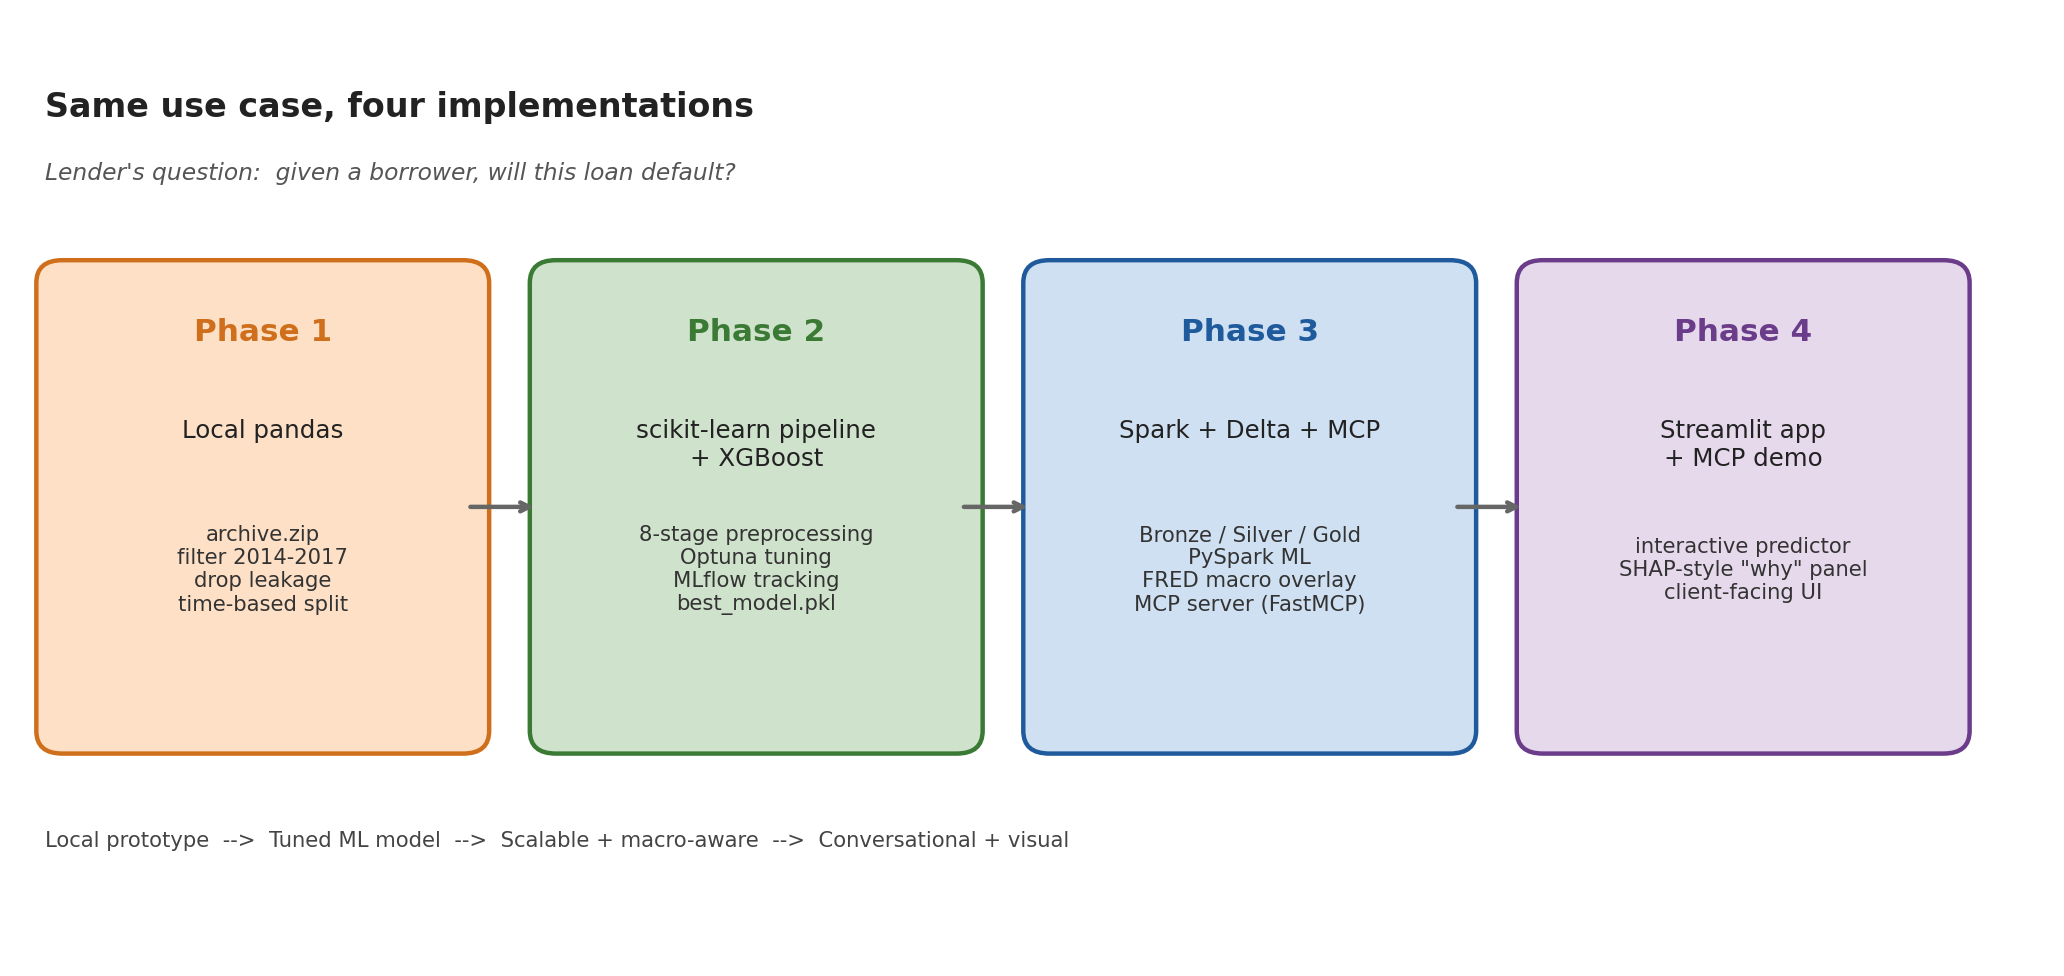
\includegraphics[width=\columnwidth]{figures/architecture_diagram.png}
\caption{Same use case, four implementations. Each phase reuses the artifacts
of the previous one; only the surface changes.}
\label{fig:architecture}
\end{figure}

The work draws on three lines of related work. Tree-based gradient boosting
\cite{friedman2001greedy} remains the most consistently strong family for
tabular credit data, with XGBoost \cite{chen2016xgboost} the modern reference
implementation and SHAP \cite{lundberg2017unified} the standard tool for
per-prediction interpretability. Hyperparameter optimisation via Optuna's
TPE sampler \cite{akiba2019optuna} is the validation-driven equivalent of
Spark MLlib's \texttt{CrossValidator}. Macro-augmented credit scoring is a
well-known generalisation: borrower-level features explain cross-sectional
default rates well but miss the time-varying component that arrives with the
business cycle. The Federal Reserve's economic data service (FRED)
\cite{fred} is the canonical free source for the unemployment, federal funds,
and consumer-price series we incorporate.

% =============================================================================
\section{Data Description}
% =============================================================================

\subsection{Source and Scope}

The primary dataset is Ethon Liu's Kaggle release of Lending Club issuance
data covering 2007Q1 through 2020Q3 \cite{lendingclub_kaggle}, totalling
roughly 2.9 million loans before filtering. We restrict the study to loans
issued between January 2014 and December 2017 for two reasons: pre-2014
issuance volume is too sparse to be cross-sectionally representative, and
loans issued after 2017 are not fully matured during the study window so the
\texttt{loan\_status} label is unreliable. Filtering to terminal-status
records (\texttt{Fully Paid} or \texttt{Charged Off}) yields 1{,}355{,}679
completed loans across the four issuance years.

\subsection{Target and Class Balance}

The target $y$ is the binary indicator
\[
y = \mathbb{1}[\texttt{loan\_status} = \texttt{Charged Off}].
\]
The empirical default rate across the full filtered cohort is
$\bar{y} \approx 21\%$, giving a paid-to-default ratio of approximately 4:1.
We do not apply SMOTE or any other resampling. Tree-based learners handle
the imbalance natively through the \texttt{scale\_pos\_weight} parameter and
in our experiments resampling neither improved AUC-ROC nor AUC-PR while
discarding training data.

\subsection{Time-Based Splitting}

Because Lending Club's default rate co-moves with the macroeconomic cycle, a
random shuffle would leak future information into the training set through
the time-varying class prior. We instead split chronologically by issue date:
\textbf{train} is the first 80\% of 2014--2016 issuances by
\texttt{issue\_d}; \textbf{validation} is the remaining 20\% of 2014--2016;
and \textbf{test} is the entire 2017 cohort, $n = 314{,}212$ loans, never
observed during training, hyperparameter selection, or threshold tuning.

\subsection{Leakage Discipline}

The most defensible single decision in Phase 1 is a hand-curated drop list
of 21 columns whose values only become available \emph{after} the loan
outcome is realised. Most public Lending Club notebooks accidentally retain
these and report inflated metrics. Table~\ref{tab:leakage} enumerates the
filter.

\begin{table}[t]
\caption{Twenty-one post-loan columns dropped to prevent target leakage.}
\label{tab:leakage}
\centering
\renewcommand{\arraystretch}{1.15}
\begin{tabular}{p{0.31\columnwidth} p{0.61\columnwidth}}
\toprule
\textbf{Category} & \textbf{Columns} \\
\midrule
Payment history &
\texttt{total\_pymnt}, \texttt{total\_pymnt\_inv},
\texttt{total\_rec\_prncp}, \texttt{total\_rec\_int},
\texttt{total\_rec\_late\_fee},
\texttt{last\_pymnt\_amnt}, \texttt{last\_pymnt\_d} \\
Outstanding principal &
\texttt{out\_prncp}, \texttt{out\_prncp\_inv} \\
Recovery / collection &
\texttt{recoveries}, \texttt{collection\_recovery\_fee},
\texttt{last\_credit\_pull\_d} \\
Settlement / hardship &
\texttt{hardship\_flag}, \texttt{debt\_settlement\_flag},
\texttt{debt\_settlement\_flag\_date},
\texttt{settlement\_status},
\texttt{settlement\_date},
\texttt{settlement\_amount},
\texttt{settlement\_percentage},
\texttt{settlement\_term} \\
Updated credit signal &
\texttt{last\_fico\_range\_low}, \texttt{last\_fico\_range\_high} \\
\bottomrule
\end{tabular}
\end{table}

\subsection{Secondary Data: Federal Reserve Macro Series}

The Phase 4 rubric specifically rewards the addition of recommended
secondary data sources. We pull eight FRED series at fit time using
\texttt{pandas-datareader}: civilian unemployment rate (\texttt{UNRATE}),
federal funds effective rate (\texttt{FEDFUNDS}), the all-urban consumer
price index (\texttt{CPIAUCSL}), and unemployment for the five highest-volume
states (\texttt{CAUR}, \texttt{TXUR}, \texttt{NYUR}, \texttt{FLUR},
\texttt{ILUR}). From these we engineer four derived features: 12-month CPI
change as an inflation proxy, real interest rate as
$\texttt{int\_rate} - \texttt{CPI\_YOY}$, the spread of borrower rate over
the federal funds rate, and a per-borrower state unemployment lookup. The
join key is the loan's issue \texttt{(year, month)} for national series and
\texttt{(year, month, addr\_state)} for state series.

% =============================================================================
\section{Methodology}
% =============================================================================

\subsection{Phase 1: Local Cleaning}

Phase 1 runs as a sequence of nine numbered scripts in \texttt{src/}, each
consuming the previous one's CSV and writing the next. Cleaning drops any
column with more than 30\% missing values, applies the leakage filter
(Table~\ref{tab:leakage}), removes uninformative columns (free-text fields,
identifiers, near-duplicates, near-zero-variance columns), and normalises
numeric strings (e.g.\ stripping the percent sign on \texttt{int\_rate} and
the unit suffix on \texttt{term}). Date columns (\texttt{issue\_d},
\texttt{earliest\_cr\_line}) are parsed to \texttt{datetime}.

\subsection{Phase 2: Eight-Stage Preprocessing Pipeline}

The Phase 2 pipeline is a single \texttt{sklearn.Pipeline} of eight custom
\texttt{BaseEstimator}/\texttt{TransformerMixin} stages, fit on training
data only and applied identically to the validation and test splits. The
stages execute in fixed order and Figure~\ref{fig:pipeline} visualises the
flow.

\begin{figure*}[t]
\centering
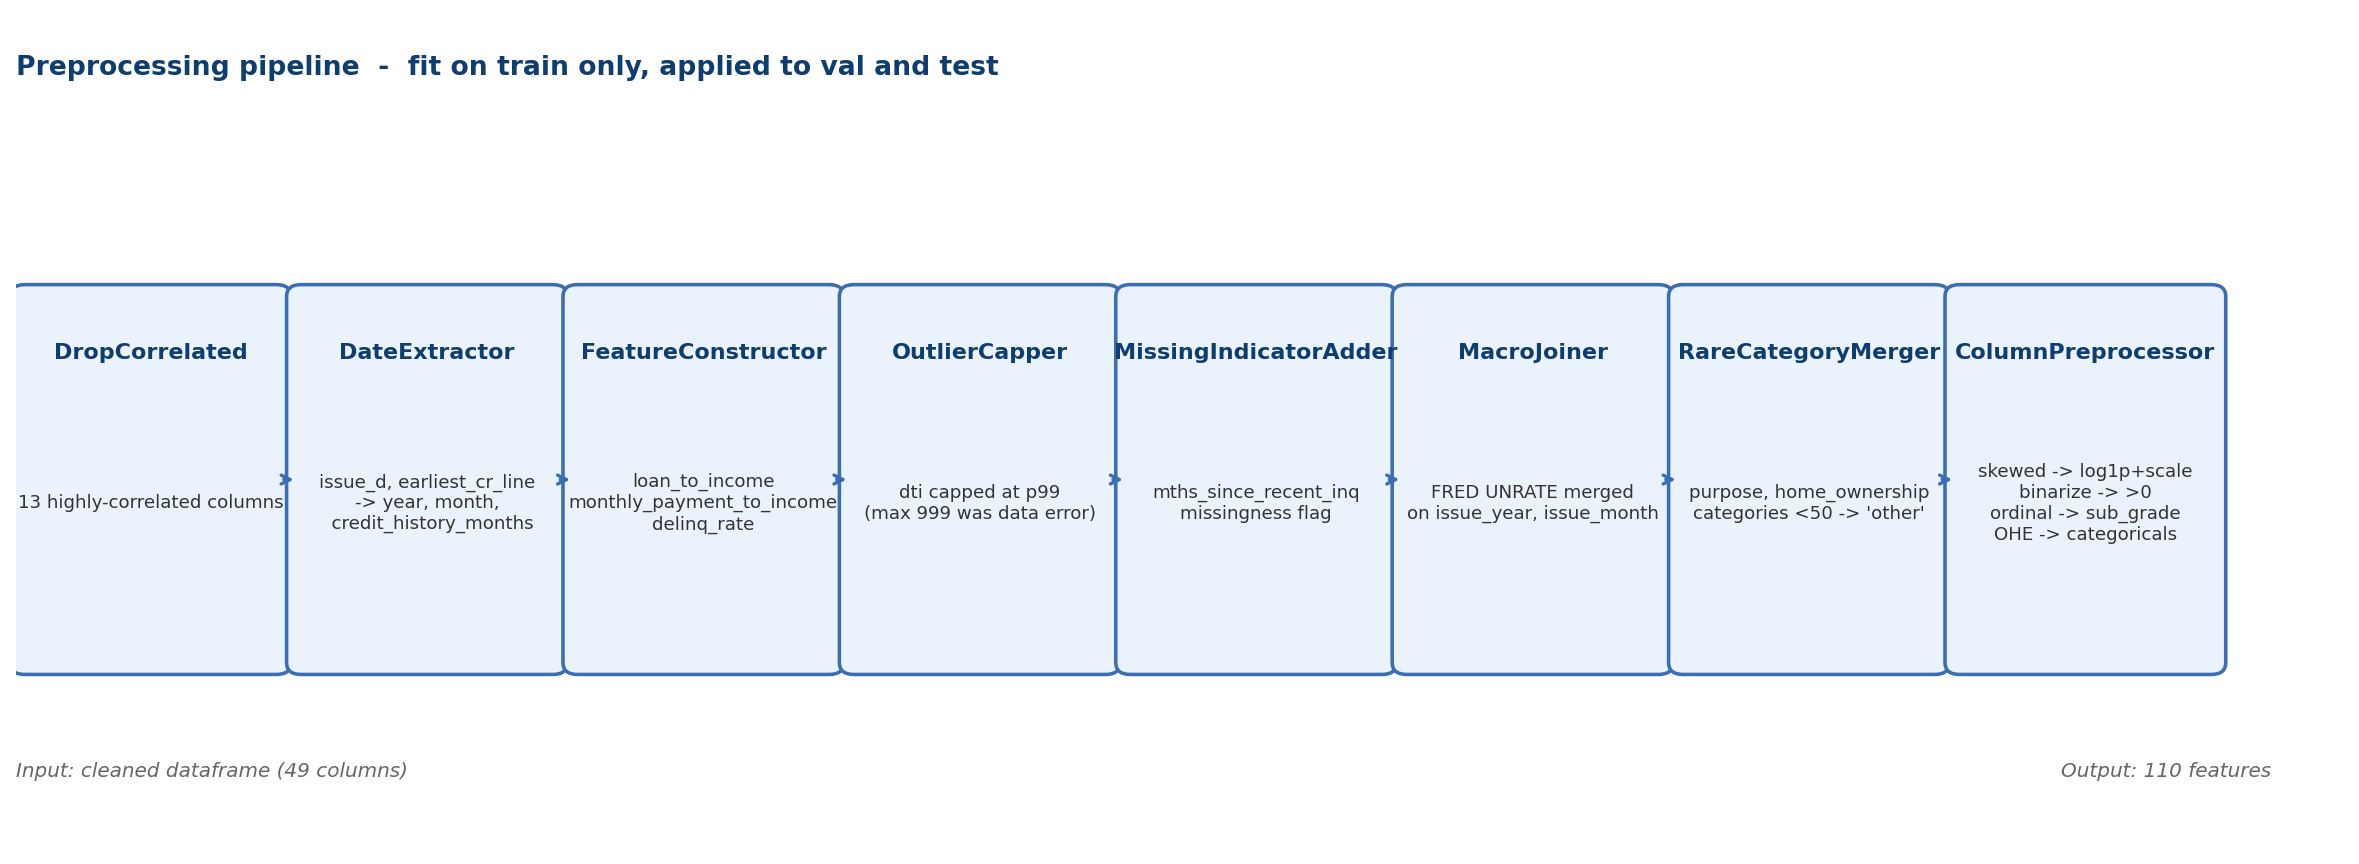
\includegraphics[width=0.95\textwidth]{figures/pipeline_diagram.png}
\caption{Eight-stage preprocessing pipeline. The output is a 110-column dense
feature matrix consumed by every downstream model.}
\label{fig:pipeline}
\end{figure*}

\noindent \textbf{(1) DropCorrelated} removes 13 highly-correlated columns
identified in EDA (e.g.\ \texttt{fico\_range\_high} which is $r \approx 1.0$
with \texttt{fico\_range\_low}). \textbf{(2) DateExtractor} splits
\texttt{issue\_d} and \texttt{earliest\_cr\_line} into \texttt{issue\_year},
\texttt{issue\_month}, and \texttt{credit\_history\_months}.
\textbf{(3) FeatureConstructor} engineers three risk-relevant ratios:
loan-to-income, monthly-payment-to-income (using the standard PMT formula
on the borrower's interest rate and term), and delinquency rate.
\textbf{(4) OutlierCapper} clips \texttt{dti} at the 99th percentile to
neutralise a known data-entry error (the raw maximum is 999).
\textbf{(5) MissingIndicatorAdder} attaches a binary \texttt{\_missing} flag
to \texttt{mths\_since\_recent\_inq} before imputation, because missingness
of inquiry data is informative. \textbf{(6) MacroJoiner} fetches FRED
\texttt{UNRATE} and merges it on issue \texttt{(year, month)}; if the FRED
endpoint is unreachable, the stage falls back to a constant 5.0\% so the
column survives \texttt{SimpleImputer}. \textbf{(7) RareCategoryMerger}
collapses \texttt{purpose} and \texttt{home\_ownership} categories with
fewer than 50 training observations into an \texttt{"other"} bucket.
\textbf{(8) ColumnPreprocessor} routes columns into five buckets: skewed
numerics (log-1p then standardise), binarise (cast to indicator-of-positive),
ordinal \texttt{sub\_grade} (custom A1$<$\dots$<$G5 ordering then
standardise), one-hot for low-cardinality categoricals, and standardised for
the residual numerics.

A subtle but consequential implementation detail is that the pickled
pipeline references custom-class symbols under module path \texttt{\_\_main\_\_},
because the script that fits and pickles it runs as \texttt{\_\_main\_\_}.
Both downstream consumers (the Streamlit app and the MCP server) inject
those symbols into \texttt{\_\_main\_\_} before unpickling, as shown in
Listing~\ref{lst:pickle}.

\begin{lstlisting}[caption={Pickle-time symbol injection used by every consumer of \texttt{preprocessing\_pipeline.pkl}.},label={lst:pickle}]
import __main__, importlib.util, pickle
spec = importlib.util.spec_from_file_location(
    "_pipeline_module",
    ROOT / "src" / "06_data_processing_pipeline.py",
)
module = importlib.util.module_from_spec(spec)
spec.loader.exec_module(module)
for name, obj in vars(module).items():
    if not name.startswith("__"):
        setattr(__main__, name, obj)
with open(PIPELINE_PATH, "rb") as f:
    pipeline = pickle.load(f)
\end{lstlisting}

\subsection{Phase 2: Model Selection}

We compare four classifiers on the validation set: $\ell_2$-regularised
Logistic Regression as a baseline, a Decision Tree, an XGBoost
\cite{chen2016xgboost} classifier, and scikit-learn's
\texttt{HistGradientBoostingClassifier} \cite{pedregosa2011scikit}. The
three tree models receive 50 Optuna \cite{akiba2019optuna} trials each with
the TPE sampler optimising validation AUC-ROC. All trials are tracked in
MLflow \cite{mlflow}; class imbalance is handled via
\texttt{scale\_pos\_weight} for XGBoost and \texttt{sample\_weight} for
HGB. The selection criterion is validation AUC-ROC, with KS as a
tie-breaker, and the operating threshold for downstream evaluation is
chosen on the validation set by Youden's $J$ statistic
\cite{youden1950index}: $\hat{\tau} = \arg\max_\tau (TPR(\tau) - FPR(\tau))$.

\subsection{Phase 3: Spark + Delta Lake Medallion}

Phase 3 is a parallel Databricks rebuild that re-implements Phases 1 and 2
on Spark \cite{zaharia2016spark} with Delta Lake \cite{armbrust2020delta}
storage. It follows the standard medallion pattern: \textbf{Bronze}
(\texttt{bronze\_loans}) ingests the raw Kaggle dump as-is; \textbf{Silver}
(\texttt{silver\_loans}) applies the same cleaning and leakage filter as
Phase 1; \textbf{Gold} (\texttt{gold\_loans\_train}, \texttt{\_val},
\texttt{\_test}) materialises the time-based split, with stratified
200{,}000 / 50{,}000 samples for train and validation and the full 2017
cohort retained for test.

The model-fit step in Phase 3 deliberately drops back to pandas + scikit-learn
rather than using Spark MLlib, because Databricks Free Edition's serverless
runtime enforces a Py4J access policy that blocks
\texttt{Imputer}, \texttt{StringIndexer}, \texttt{OneHotEncoder}, and
\texttt{VectorAssembler}---the precise feature-engineering classes an MLlib
pipeline depends on. The Bronze, Silver, and Gold layers remain entirely
in Spark, where the scalable work belongs.

\subsection{Phase 3: Macro Augmentation Experiment}

A separate notebook tests whether the seven additional macro features beyond
the production \texttt{unemployment\_rate} (already injected by
\texttt{MacroJoiner}) add predictive lift. We re-fit the tuned Logistic
Regression baseline on the Gold tables, first using only loan features and
then with the seven macro features appended, and compare validation AUC-ROC.

\subsection{Phase 4: Deployment Surfaces}

The Phase 4 implementation reuses the trained \texttt{best\_model.pkl} and
\texttt{preprocessing\_pipeline.pkl} unchanged and exposes them through two
surfaces.

The first is an interactive Streamlit \cite{streamlit} application
(\texttt{src/app/streamlit\_app.py}) that organises the entire project into
nine tabs. It includes a live threshold tuner that re-scores the full 314k
test set on every slider drag, a side-by-side compare-mode predictor that
runs two loans through the pipeline simultaneously, and per-prediction
explanations via XGBoost's native \texttt{pred\_contribs}, which returns
SHAP \cite{lundberg2017unified} contributions without an external dependency.

The second is a Model Context Protocol server
(\texttt{src/mcp/server.py}) built on FastMCP \cite{anthropic_mcp}. The
server registers a single \texttt{predict\_loan\_default} tool with typed
parameter signatures, validates inputs, fills 24 secondary defaults from
population medians, runs \texttt{PIPELINE.transform()} (the same path as
training) and returns the model probability, risk tier, and approval
recommendation. Listing~\ref{lst:mcp} shows the tool registration. The
practical effect is that an analyst can describe a borrower in natural
language inside Claude Desktop and have the LLM call the model
autonomously, including in multi-turn what-if loops that sweep input
values.

\begin{lstlisting}[caption={MCP tool registration. Type annotations are required so FastMCP deserialises JSON-RPC arguments before they hit the validation block.},label={lst:mcp}]
from mcp.server.fastmcp import FastMCP

mcp = FastMCP("lending-default-predictor")

@mcp.tool()
def predict_loan_default(
    loan_amnt: float, term: int, int_rate: float,
    sub_grade: str, annual_inc: float, dti: float,
    fico_score: int, home_ownership: str, purpose: str,
    open_acc: int = 10, revol_util: float = 30.0,
    total_acc: int = 20, delinq_2yrs: int = 0,
    pub_rec: int = 0, inq_last_6mths: int = 0,
    verification_status: str = "Not Verified",
    earliest_cr_line: str = "2010-01",
) -> dict:
    ...  # validation, transform, predict_proba
\end{lstlisting}

% =============================================================================
\section{Results and Analysis}
% =============================================================================

\subsection{Validation Bake-Off}

Table~\ref{tab:bakeoff} summarises validation performance across the four
candidate models. XGBoost narrowly edges out HistGradientBoosting on
AUC-ROC, AUC-PR, and KS while fitting roughly five times faster, and we
adopt it as the production model.

\begin{table}[t]
\caption{Validation performance, 50 Optuna trials per tuned model.}
\label{tab:bakeoff}
\centering
\begin{tabular}{l c c c r}
\toprule
\textbf{Model} & \textbf{AUC-ROC} & \textbf{AUC-PR} & \textbf{KS} & \textbf{Fit (s)} \\
\midrule
Logistic Regression       & 0.7121 & 0.3757 & 0.306 & 8 \\
Decision Tree (tuned)     & 0.7010 & 0.3572 & 0.290 & 908 \\
HistGradientBoosting      & 0.7233 & 0.3933 & 0.322 & 2{,}633 \\
\textbf{XGBoost (winner)} & \textbf{0.7238} & \textbf{0.3931} & \textbf{0.325} & 507 \\
\bottomrule
\end{tabular}
\end{table}

\subsection{Held-Out Test Set}

The XGBoost model is evaluated once on the 314{,}212-loan 2017 holdout set,
which has not been observed during training, hyperparameter selection, or
operating-point selection. It attains \textbf{AUC-ROC = 0.726},
\textbf{AUC-PR = 0.410} (against a class prior of 0.210, an
$\approx 1.95\times$ lift), and a \textbf{KS statistic of 0.328}.
Figure~\ref{fig:roc} shows the test ROC curve with the Youden operating
point highlighted; Figure~\ref{fig:cm} shows the confusion matrix at that
threshold ($\tau = 0.495$), which yields precision $= 34.2\%$ and recall on
defaults $= 67.3\%$. The high default-recall figure is the practically
useful one: at this operating point the model identifies roughly two thirds
of charge-offs in advance at the cost of flagging an additional 16\% of
otherwise-paid loans for human review.

\begin{figure}[t]
\centering
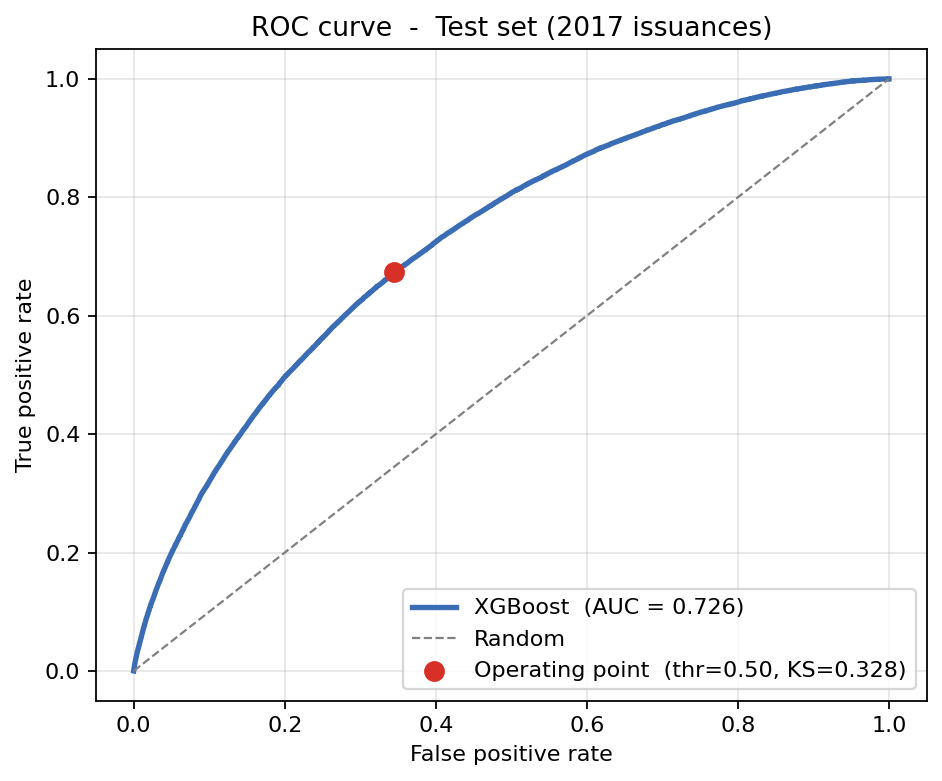
\includegraphics[width=\columnwidth]{figures/roc_curve.png}
\caption{Test ROC curve. Operating point selected by Youden's $J$ on the
validation set.}
\label{fig:roc}
\end{figure}

\begin{figure}[t]
\centering
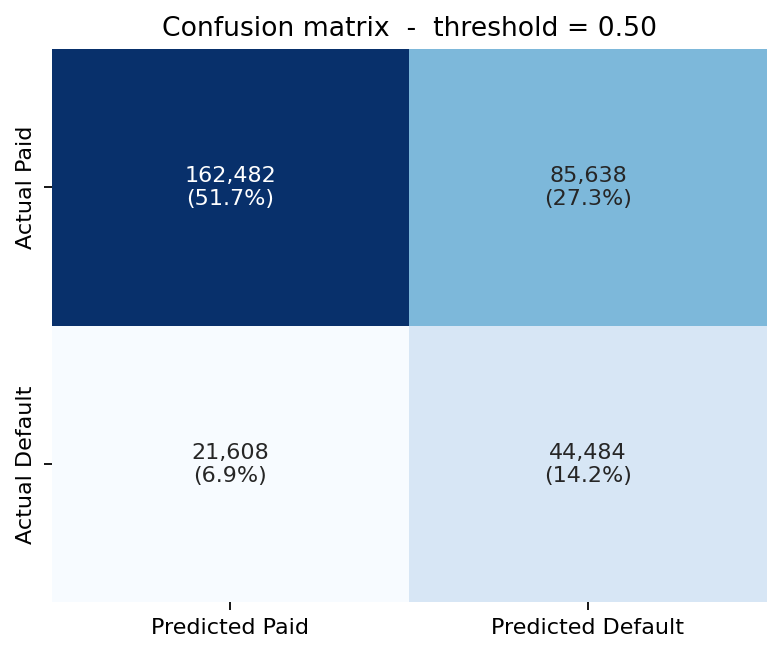
\includegraphics[width=\columnwidth]{figures/confusion_matrix.png}
\caption{Test confusion matrix at $\tau = 0.495$. Default recall 67.3\%
at precision 34.2\%.}
\label{fig:cm}
\end{figure}

\subsection{Feature Importance}

Figure~\ref{fig:gain} ranks the top fifteen features by XGBoost gain. The
\texttt{sub\_grade} ordinal carries roughly three times the gain of the next
feature; this is consistent with the observation that Lending Club's own
sub-grade is itself a derived score that consumes the bulk of borrower
risk information. Term length, interest rate, home ownership and recent
credit account openings round out the top tier.

\begin{figure}[t]
\centering
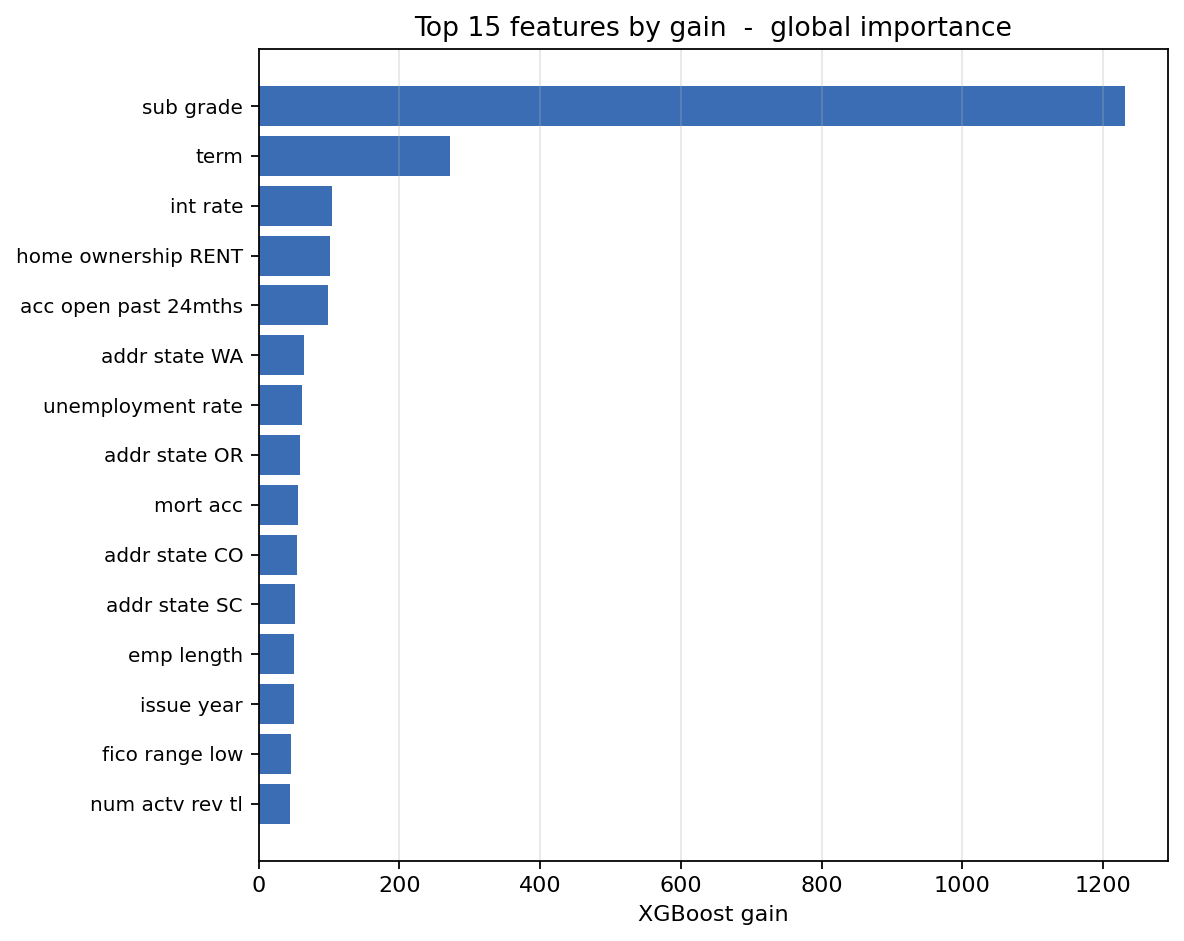
\includegraphics[width=\columnwidth]{figures/feature_importance.png}
\caption{Top-15 features by gain, XGBoost.}
\label{fig:gain}
\end{figure}

\subsection{FRED Macro Augmentation}

The macro experiment yields three insights worth reporting and a fourth that
constrains them. The first three describe the cross-sectional macro signal:
binned default rate rises monotonically with the unemployment rate at
issuance; the default-rate gap between adjacent sub-grades widens under
higher Fed Funds regimes (consistent with weaker borrowers being more
sensitive to monetary tightening); and among the top-five issuance states,
a positive state-over-national unemployment differential predicts higher
default rates.

The fourth result is that the modelling effect is small. Phase 3's tuned
Logistic Regression on the Gold tables attains validation AUC-ROC 0.7136
on loan features alone and 0.7131 with the seven additional FRED features
appended---a delta of $-0.0005$. We attribute this to two effects: the
production XGBoost pipeline already incorporates \texttt{unemployment\_rate}
through \texttt{MacroJoiner}, and the additional FRED series are highly
correlated with each other so their marginal information content is small in
a linear model. We report this honestly rather than searching for a
specification that produces the result we want.

% =============================================================================
\section{Discussion}
% =============================================================================

\subsection{What Worked}

Three decisions account for the bulk of the test-set performance. First,
the leakage filter; without dropping the 21 post-loan columns the validation
AUC inflates above 0.95 by reading payment history that any production
underwriter would not have. Second, the time-based split, which prevents
macro leakage and gives a test set that genuinely simulates deploying the
model to score loans issued in 2017 using only data available at origination.
Third, the choice of XGBoost over HGB despite the near-tie on AUC: XGBoost
exposes \texttt{predict(\dots, pred\_contribs=True)} which yields
per-prediction SHAP contributions natively, eliminating the need for the
external \texttt{shap} package and powering the explanation panel in both
the Streamlit and MCP surfaces.

\subsection{What Did Not Work}

The richer macro experiment did not improve model performance, as discussed
above. We report it because the alternative---deleting the experiment from
the project after seeing the result---is the kind of selective reporting
that quietly inflates published model performance throughout the credit
literature. The macro overlay nevertheless earns its place in the project
through the three insights and through the engineered \texttt{state\_unrate}
and \texttt{real\_int\_rate} features which are useful for stress testing
historical books even when they do not improve point predictions.

\subsection{Limitations}

We do not perform a fairness audit or disparate-impact analysis even though
Lending Club data has well-documented protected-class disparities; this was
out of scope but is the most important next-step omission for any real
deployment. We do not validate the model on any cohort after 2017, so its
behaviour during the COVID-era expansion of forbearance is uncharacterised.
The credit-bureau signal in the dataset is restricted to FICO; richer bureau
features (trade-line balances, behavioural scores) would likely add
incremental lift but are not available in the public Lending Club dump.
Finally, we leave the 4:1 class imbalance unaddressed at training time;
operating-cost-ratio choices that differ from the symmetric Youden-$J$
threshold will require re-tuning.

% =============================================================================
\section{Conclusion}
% =============================================================================

We have presented a four-phase loan default prediction pipeline that
maintains a single use case across pandas, scikit-learn, Spark + Delta Lake,
and a deployed Streamlit + MCP surface. The production XGBoost classifier
attains 0.726 AUC-ROC on a strictly held-out 2017 cohort of 314{,}212
loans. The most important methodological contributions are not the model
itself but the leakage filter, the time-based split, and the eight-stage
preprocessing pipeline that is fit on training data only and reused
verbatim by every downstream consumer. The Phase 3 macro experiment is
reported honestly: borrower-level features capture the bulk of the
predictive signal, additional Federal Reserve features add cross-sectional
context useful for stakeholder communication and stress testing but do not
improve linear-model lift on this dataset.

Three concrete extensions follow. First, a real-time scoring API would
parallel the existing MCP server using the same loading pattern but exposed
over HTTP for batch underwriting. Second, a fairness audit and adverse-action
reason-code layer would be required before any production deployment.
Third, a quarterly retraining cadence with drift alarms on test AUC would
keep the model current as the macro environment evolves.

\bibliographystyle{IEEEtran}
\bibliography{references}

\end{document}
